\WarningFilter{latex}{Text page 31 contains only floats}

\begin{figure*}[tb!]
    \centering
    \begin{subfigure}[b]{0.2\textwidth}
        \centering
        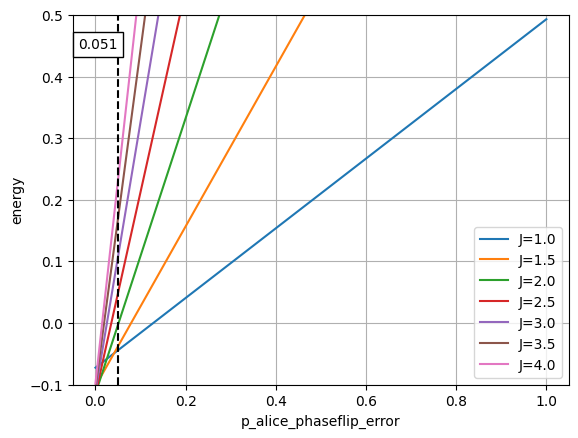
\includegraphics[width=\textwidth]{Appendix/plots/errors/numerical/Alice/N1/N1_energy_vs_p_alice_phaseflip_error.png}
        \caption{Energy, $N=1$}
    \end{subfigure}
    \hfill
    \begin{subfigure}[b]{0.2\textwidth}
        \centering
        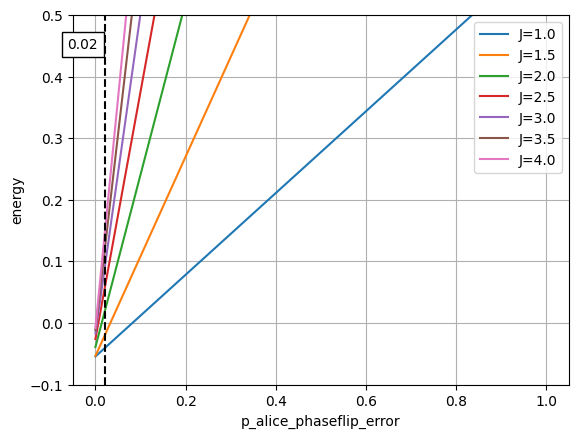
\includegraphics[width=\textwidth]{Appendix/plots/errors/numerical/Alice/N2/N2_energy_vs_p_alice_phaseflip_error.png}
        \caption{Energy, $N=2$}
    \end{subfigure}
    \hfill
    \begin{subfigure}[b]{0.2\textwidth}
        \centering
        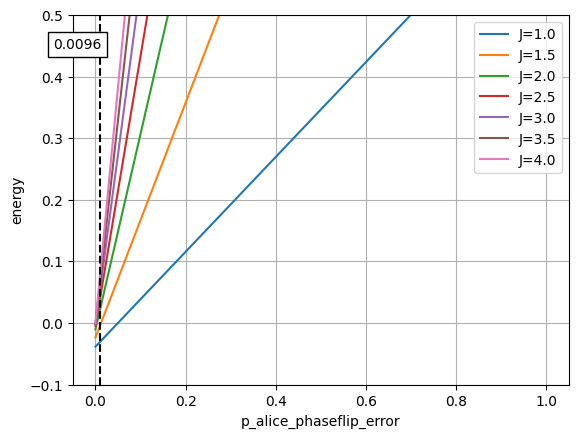
\includegraphics[width=\textwidth]{Appendix/plots/errors/numerical/Alice/N3/N3_energy_vs_p_alice_phaseflip_error.png}
        \caption{Energy, $N=3$}
    \end{subfigure}
    \hfill
    \begin{subfigure}[b]{0.2\textwidth}
        \centering
        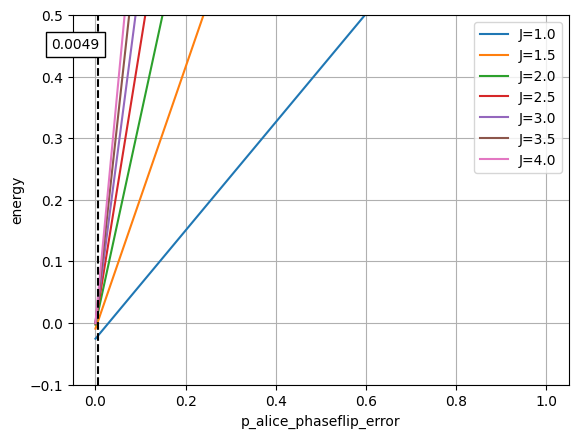
\includegraphics[width=\textwidth]{Appendix/plots/errors/numerical/Alice/N4/N4_energy_vs_p_alice_phaseflip_error.png}
        \caption{Energy, $N=4$}
    \end{subfigure}

    \vspace{0.5em}

    \begin{subfigure}[b]{0.2\textwidth}
        \centering
        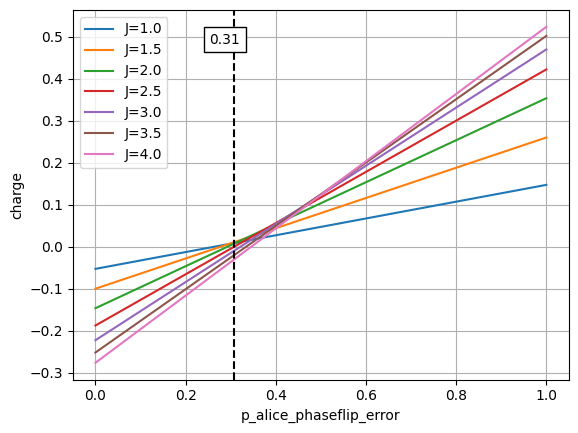
\includegraphics[width=\textwidth]{Appendix/plots/errors/numerical/Alice/N1/N1_charge_vs_p_alice_phaseflip_error.png}
        \caption{Charge, $N=1$}
    \end{subfigure}
    \hfill
    \begin{subfigure}[b]{0.2\textwidth}
        \centering
        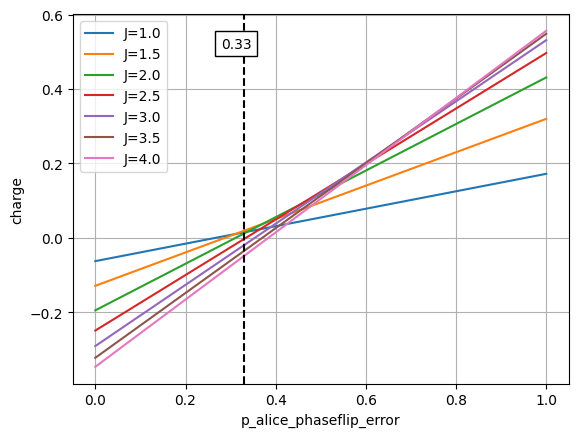
\includegraphics[width=\textwidth]{Appendix/plots/errors/numerical/Alice/N2/N2_charge_vs_p_alice_phaseflip_error.png}
        \caption{Charge, $N=2$}
    \end{subfigure}
    \hfill
    \begin{subfigure}[b]{0.2\textwidth}
        \centering
        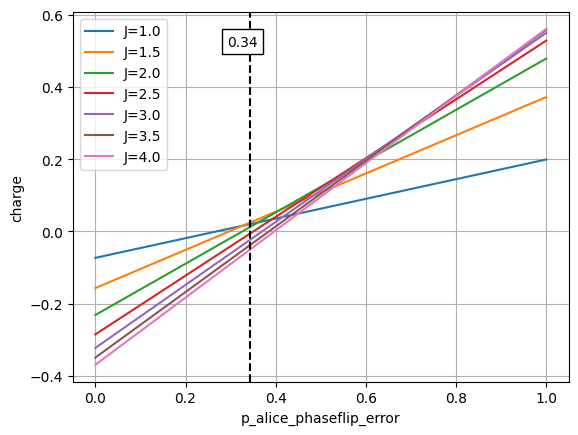
\includegraphics[width=\textwidth]{Appendix/plots/errors/numerical/Alice/N3/N3_charge_vs_p_alice_phaseflip_error.png}
        \caption{Charge, $N=3$}
    \end{subfigure}
    \hfill
    \begin{subfigure}[b]{0.2\textwidth}
        \centering
        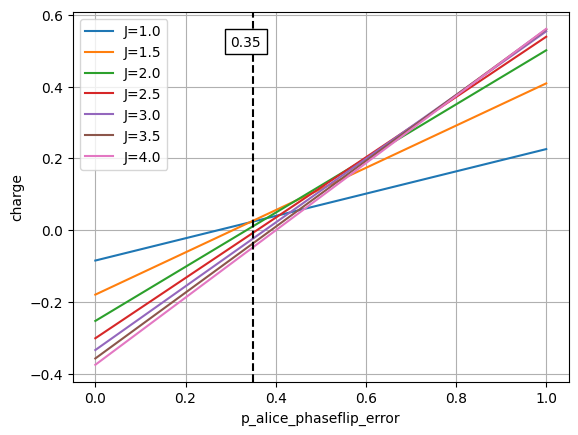
\includegraphics[width=\textwidth]{Appendix/plots/errors/numerical/Alice/N4/N4_charge_vs_p_alice_phaseflip_error.png}
        \caption{Charge, $N=4$}
    \end{subfigure}
    
    \caption{Numerical simulation results for teleported expectation value vs. the probability $p$ of phaseflip at Alice's site for Star-Interaction Hamiltonian \(H^{(1)}\).}
    \label{fig:alice_num_alice_phaseflip_error_appendix}
\end{figure*}

\begin{figure*}[tb!]
    \centering
    \begin{subfigure}[b]{0.33\textwidth}
        \centering
        
\includegraphics[width=\textwidth]{Appendix/plots/errors/qiskit/Alice/N1/N1_energy_vs_p_alice_phaseflip_error.png}
        \caption{Energy, $N=1$}
    \end{subfigure}
    \hfill
    \begin{subfigure}[b]{0.33\textwidth}
        \centering
        
\includegraphics[width=\textwidth]{Appendix/plots/errors/qiskit/Alice/N2/N2_energy_vs_p_alice_phaseflip_error.png}
        \caption{Energy, $N=2$}
    \end{subfigure}
    \hfill
    \begin{subfigure}[b]{0.33\textwidth}
        \centering
        
\includegraphics[width=\textwidth]{Appendix/plots/errors/qiskit/Alice/N3/N3_energy_vs_p_alice_phaseflip_error.png}
        \caption{Energy, $N=3$}
    \end{subfigure}

    \vspace{0.5em}

    \begin{subfigure}[b]{0.33\textwidth}
        \centering
        
\includegraphics[width=\textwidth]{Appendix/plots/errors/qiskit/Alice/N1/N1_charge_vs_p_alice_phaseflip_error.png}
        \caption{Charge, $N=1$}
    \end{subfigure}
    \hfill
    \begin{subfigure}[b]{0.33\textwidth}
        \centering
        
\includegraphics[width=\textwidth]{Appendix/plots/errors/qiskit/Alice/N2/N2_charge_vs_p_alice_phaseflip_error.png}
        \caption{Charge, $N=2$}
    \end{subfigure}
    \hfill
    \begin{subfigure}[b]{0.33\textwidth}
        \centering
        
\includegraphics[width=\textwidth]{Appendix/plots/errors/qiskit/Alice/N3/N3_charge_vs_p_alice_phaseflip_error.png}
        \caption{Charge, $N=3$}
    \end{subfigure}
    
    \caption{Qiskit simulation results for teleported expectation value vs. the probability $p$ of phaseflip at Alice's site for Star-Interaction Hamiltonian \(H^{(1)}\).}
    \label{fig:alice_qiskit_alice_phaseflip_error_appendix}
\end{figure*}

\begin{figure*}[tb!]
    \centering
    \begin{subfigure}[b]{0.29\textwidth}
        \centering
        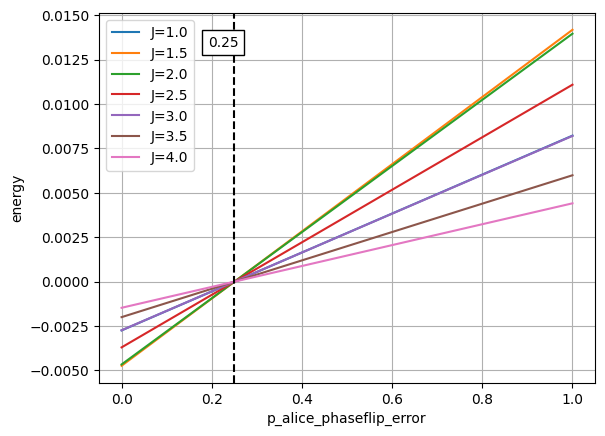
\includegraphics[width=\textwidth]{Appendix/plots/errors/numerical/NearestNeighbors/N2/X_N2_energy_vs_p_alice_phaseflip_error.png}
        \caption{Energy, $N=2$}
    \end{subfigure}
    \hfill
    \begin{subfigure}[b]{0.29\textwidth}
        \centering
        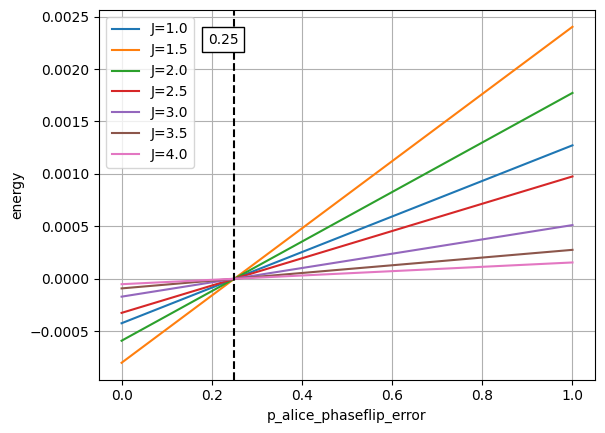
\includegraphics[width=\textwidth]{Appendix/plots/errors/numerical/NearestNeighbors/N3/X_N3_energy_vs_p_alice_phaseflip_error.png}
        \caption{Energy, $N=3$}
    \end{subfigure}
    \hfill
    \begin{subfigure}[b]{0.29\textwidth}
        \centering
        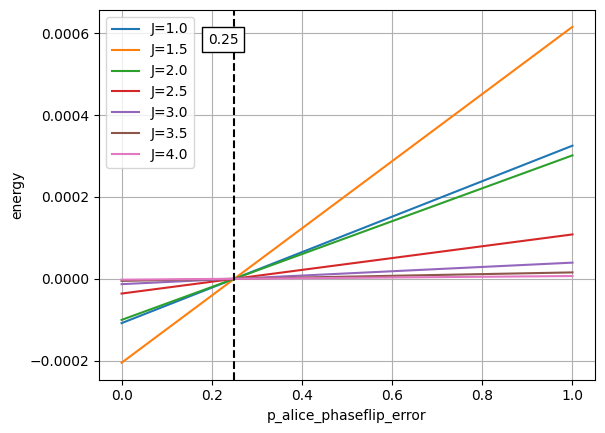
\includegraphics[width=\textwidth]{Appendix/plots/errors/numerical/NearestNeighbors/N4/X_N4_energy_vs_p_alice_phaseflip_error.png}
        \caption{Energy, $N=4$}
    \end{subfigure}

    \vspace{0.5em}

    \begin{subfigure}[b]{0.29\textwidth}
        \centering
        
\includegraphics[width=\textwidth]{plots/errors/numerical/N2_charge_vs_p_alice_phaseflip_error.png}
        \caption{Charge, $N=2$}
    \end{subfigure}
    \hfill
    \begin{subfigure}[b]{0.29\textwidth}
        \centering
        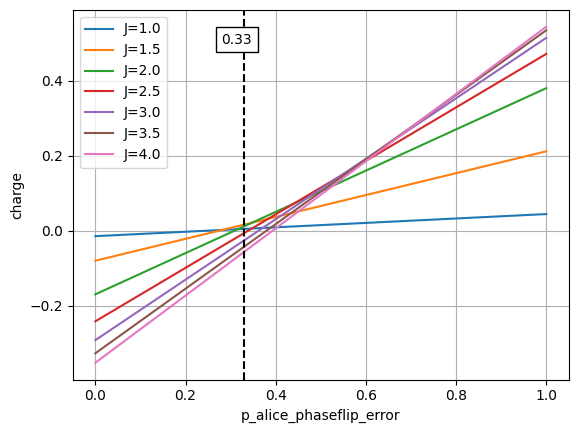
\includegraphics[width=\textwidth]{Appendix/plots/errors/numerical/NearestNeighbors/N3/X_N3_charge_vs_p_alice_phaseflip_error.png}
        \caption{Charge, $N=3$}
    \end{subfigure}
    \hfill
    \begin{subfigure}[b]{0.29\textwidth}
        \centering
        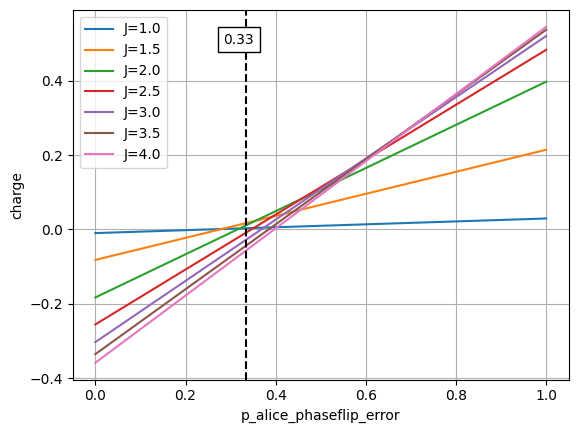
\includegraphics[width=\textwidth]{Appendix/plots/errors/numerical/NearestNeighbors/N4/X_N4_charge_vs_p_alice_phaseflip_error.png}
        \caption{Charge, $N=4$}
    \end{subfigure}
    
    \caption{Numerical simulation results for teleported expectation value vs. the probability $p$ of phaseflip at Alice's site for Nearest Neighbors Hamiltonian \(H^{(2)}\) with Alice base \(\sigma_A = X_0\).}
    \label{fig:nn_X_num_alice_phaseflip_error_appendix}
\end{figure*}

\begin{figure*}[tb!]
    \centering
    \begin{subfigure}[b]{0.29\textwidth}
        \centering
        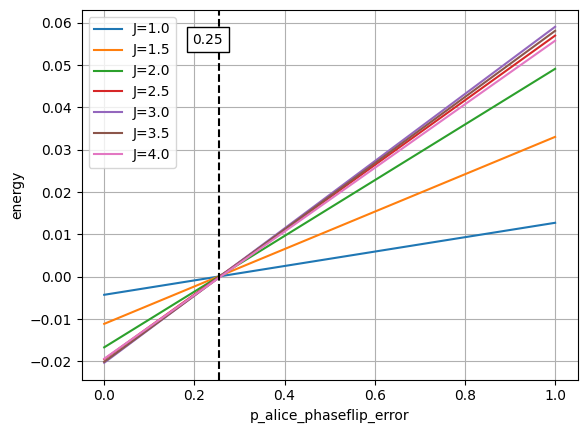
\includegraphics[width=\textwidth]{Appendix/plots/errors/numerical/NearestNeighbors/N2/Y_N2_energy_vs_p_alice_phaseflip_error.png}
        \caption{Energy, $N=2$}
    \end{subfigure}
    \hfill
    \begin{subfigure}[b]{0.29\textwidth}
        \centering
        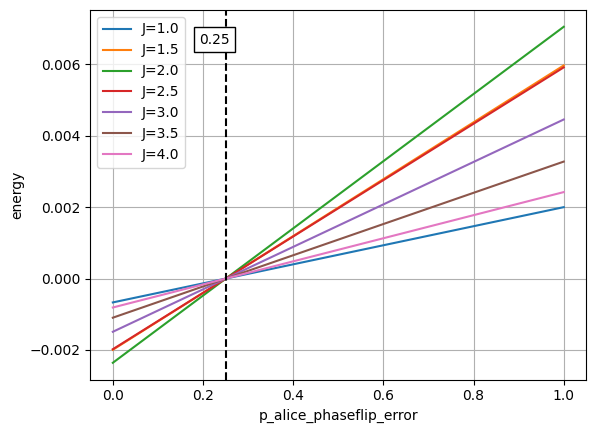
\includegraphics[width=\textwidth]{Appendix/plots/errors/numerical/NearestNeighbors/N3/Y_N3_energy_vs_p_alice_phaseflip_error.png}
        \caption{Energy, $N=3$}
    \end{subfigure}
    \hfill
    \begin{subfigure}[b]{0.29\textwidth}
        \centering
        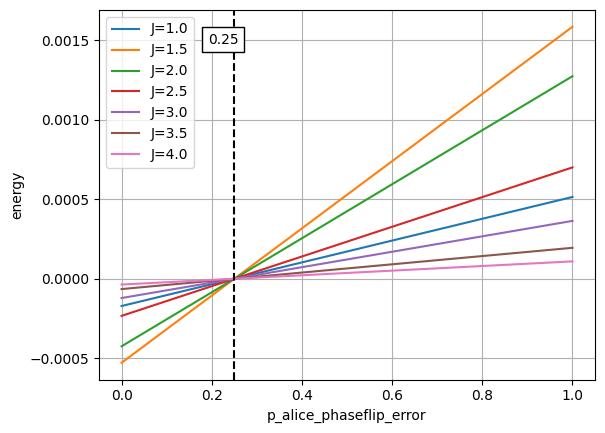
\includegraphics[width=\textwidth]{Appendix/plots/errors/numerical/NearestNeighbors/N4/Y_N4_energy_vs_p_alice_phaseflip_error.png}
        \caption{Energy, $N=4$}
    \end{subfigure}

    \vspace{0.5em}

    \begin{subfigure}[b]{0.29\textwidth}
        \centering
        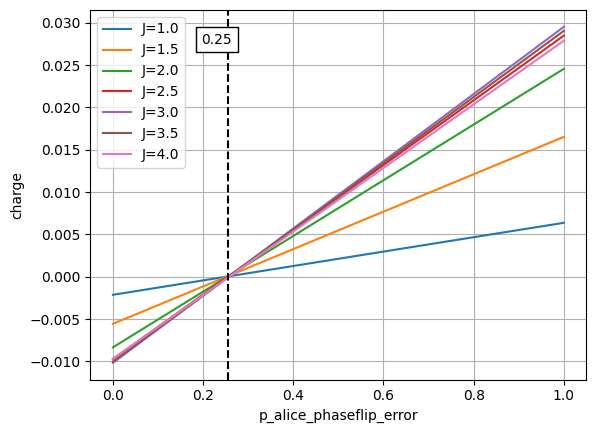
\includegraphics[width=\textwidth]{Appendix/plots/errors/numerical/NearestNeighbors/N2/Y_N2_charge_vs_p_alice_phaseflip_error.png}
        \caption{Charge, $N=2$}
    \end{subfigure}
    \hfill
    \begin{subfigure}[b]{0.29\textwidth}
        \centering
        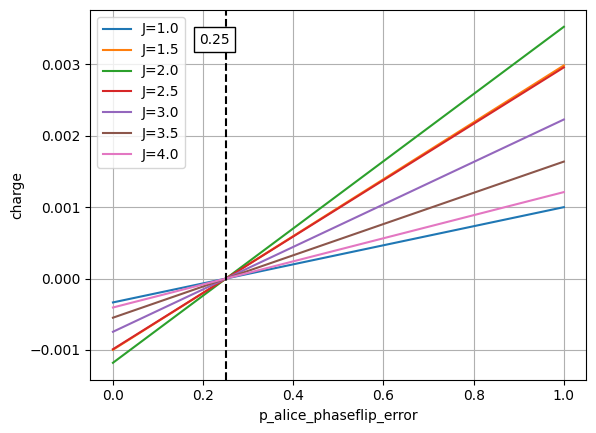
\includegraphics[width=\textwidth]{Appendix/plots/errors/numerical/NearestNeighbors/N3/Y_N3_charge_vs_p_alice_phaseflip_error.png}
        \caption{Charge, $N=3$}
    \end{subfigure}
    \hfill
    \begin{subfigure}[b]{0.29\textwidth}
        \centering
        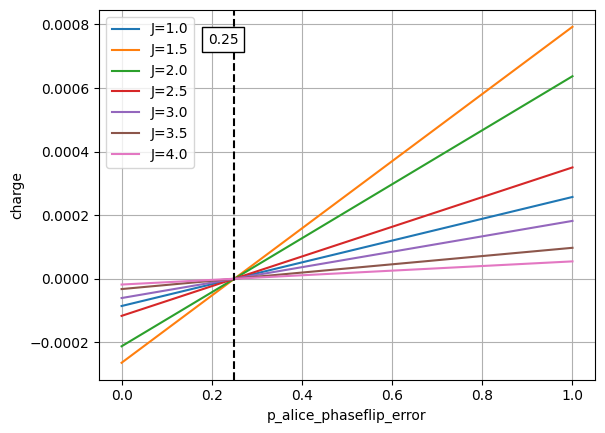
\includegraphics[width=\textwidth]{Appendix/plots/errors/numerical/NearestNeighbors/N4/Y_N4_charge_vs_p_alice_phaseflip_error.png}
        \caption{Charge, $N=4$}
    \end{subfigure}
    
    \caption{Numerical simulation results for teleported expectation value vs. the probability $p$ of phaseflip at Alice's site for Nearest Neighbors Hamiltonian \(H^{(2)}\) with Alice base \(\sigma_A = Y_0\).}
    \label{fig:nn_Y_num_alice_phaseflip_error_appendix}
\end{figure*}

\begin{figure*}[tb!]
    \centering
    \begin{subfigure}[b]{0.24\textwidth}
        \centering
        
\includegraphics[width=\textwidth]{Appendix/plots/errors/qiskit/NearestNeighbors/N2/X_N2_energy_vs_p_alice_phaseflip_error.png}
        \caption{Energy, $N=2$, $\sigma_A = X_0$}
    \end{subfigure}
    \hfill
    \begin{subfigure}[b]{0.24\textwidth}
        \centering
        
\includegraphics[width=\textwidth]{Appendix/plots/errors/qiskit/NearestNeighbors/N3/X_N3_energy_vs_p_alice_phaseflip_error.png}
        \caption{Energy, $N=3$, $\sigma_A = X_0$}
    \end{subfigure}
    \hfill
    \begin{subfigure}[b]{0.24\textwidth}
        \centering
        
\includegraphics[width=\textwidth]{plots/errors/qiskit/N2_charge_vs_p_alice_phaseflip_error.png}
        \caption{Charge, $N=2$, $\sigma_A = X_0$}
    \end{subfigure}
    \hfill
    \begin{subfigure}[b]{0.24\textwidth}
        \centering
        
\includegraphics[width=\textwidth]{Appendix/plots/errors/qiskit/NearestNeighbors/N3/X_N3_charge_vs_p_alice_phaseflip_error.png}
        \caption{Charge, $N=3$, $\sigma_A = X_0$}
    \end{subfigure}

    \vspace{0.5em}

    \begin{subfigure}[b]{0.24\textwidth}
        \centering
        
\includegraphics[width=\textwidth]{Appendix/plots/errors/qiskit/NearestNeighbors/N2/Y_N2_energy_vs_p_alice_phaseflip_error.png}
        \caption{Energy, $N=2$, $\sigma_A = Y_0$}
    \end{subfigure}
    \hfill
    \begin{subfigure}[b]{0.24\textwidth}
        \centering
        
\includegraphics[width=\textwidth]{Appendix/plots/errors/qiskit/NearestNeighbors/N3/Y_N3_energy_vs_p_alice_phaseflip_error.png}
        \caption{Energy, $N=3$, $\sigma_A = Y_0$}
    \end{subfigure}
    \hfill
    \begin{subfigure}[b]{0.24\textwidth}
        \centering
        
\includegraphics[width=\textwidth]{Appendix/plots/errors/qiskit/NearestNeighbors/N2/Y_N2_charge_vs_p_alice_phaseflip_error.png}
        \caption{Charge, $N=2$, $\sigma_A = Y_0$}
    \end{subfigure}
    \hfill
    \begin{subfigure}[b]{0.24\textwidth}
        \centering
        
\includegraphics[width=\textwidth]{Appendix/plots/errors/qiskit/NearestNeighbors/N3/Y_N3_charge_vs_p_alice_phaseflip_error.png}
        \caption{Charge, $N=3$, $\sigma_A = Y_0$}
    \end{subfigure}
    
    \caption{Qiskit simulation results for teleported expectation value vs. the probability $p$ of phaseflip at Alice's site for Nearest Neighbors Hamiltonian \(H^{(2)}\) for both Alice bases.}
    \label{fig:nn_qiskit_alice_phaseflip_error_appendix}
\end{figure*}
